\chapter{Design}

\section{Overall System Design}

\subsection{Short description of the main parts of the system}

\begin{itemize}
\item Log In Window
\item Main Database Interface
\item Adding/Removing/Editing Customers and Entries
\item Calender Interface
\item Changing Password
\item Search Window
\end{itemize}

\

Log In Window
\begin{itemize}
    \item A window is displayed which prompts the user to input their ID and password.
    \item Checks the entered valiues with the database to identify whether the user's credentials are correct.
    \item Once a correct set of values are entered, the user will be granted access to the database.
    \item A link will be at the bottom which says "Forgotten password?". This can be clicked on and then the user wil be prompted for the email address, and the corresponding password for the email address entered will be sent to that email.
    \item If there is no record of an email and password then the user will be prompted to create one for their corresponding email.
\end{itemize}

\
  
Main Database Interface
\begin{itemize}
    \item This will be the "home" interface.
    \item A view of the Customer details in the database will be available.
    \item The user can select an author from the basic view of the database, and click view
    \item A user interface is presented with a set of options which are: View, Search Database, Add Entry, Remove an Entry, Edit an Entry, Change Password, and Log out.
    \item Clicking the Search Database Button will prompt a seperate interface to open, and shows details which can be used to search for specific items in the database.

\end{itemize}

\
View Screen
\begin{itemize}
    \item Clicking view after having selected an customer will open a new window which will show a more in depth view of it. It will show the books that have been published with them.
    \item There will be buttons to expand on certain fields, including Royalties, Publishing Invoices and Book Invoices. These will show in new windows. If the user has clicked on Royalties, they have the option to click on Royalties Items on the following screen, where they can see breakdown of it. If they have clicked on Book Invoices, they can click on the Book Invoice Items on the following screen to see a breakdown of these too. From the Royalties/Book Invoice screens, they can calculate and add more Royalties/Invoices.
    \item Customers can be searched for quickly using their AuthorID on this screen.
\end{itemize}

\

Adding/Removing/Editing Customers and Entries
\begin{itemize}
    \item Clicking the Add Entry Button will prompt a seperate interface to open, and contains a layout of entry boxes for required fields for entering details about the customer. After this, the user can click on the customer's new record from the menu and click edit or a book/royalties/royalty items/book invoice/book invoice items/publication invoice, dependent on which has been selected. An existing customer can be selected using the search function.
    \item If a customer already exists, and details are needed to be edited or deleted, a search can be conducted to find that customer.
    \item Clicking the Remove Entry Button will prompt a seperate interface to open, which contains a view of the database, consisting of all the customers. Three search boxes can be used for searching for their forename, surname or AuthorID. If an entry was selected beforehand, then upon clicking Remove Entry, The user will be prompted for confirmation, then asked to enter their password. 
    \item Clicking the Edit Entry button will prompt a seperate interface to open, and will contain a view of the database. An entry can be searched for using the search, selected, and once the user clicks "Edit", the user will be prompted with a text box, asking for the user to enter text. Upon confirming what the user wants to enter, they are required to enter their password. This will then be saved. If a customer entry was selected before hand, a new window for adding entries will open first upon clicking Edit Entry, and the data about the customers will be in the fields already, ready for editing. Then, the data can be edited and saved, and the user will be prompted for confirmation then asked to enter their password.
\end{itemize}

\

Changing Password
\begin{itemize}
    \item An interface will open, which will prompt the user to enter their Email, Old Password, and Dhen the new password twice for confirmation.
    \item Once this has been confirmed, the interface will close, resorting back to the log in window.
\end{itemize}

\

Search Window
\begin{itemize}
    \item Clicking the Search Database Button will open a seperate interface, which contains a set of fields that the user can use to search the database by.
    \item Once the Search Button is clicked, a list of all the data entries that match the search criteria will come up in a list in the Main Window.
    \item The search can be refined by searching again, and an item can be selected from the search results.
\end{itemize}

\subsection{System flowcharts showing an overview of the complete system}

The following is a flowchart representing a summary of the complete system.

\begin{figure}[H]
    \caption{Flowchart 1} \label{Flowchart_1.pdf}
    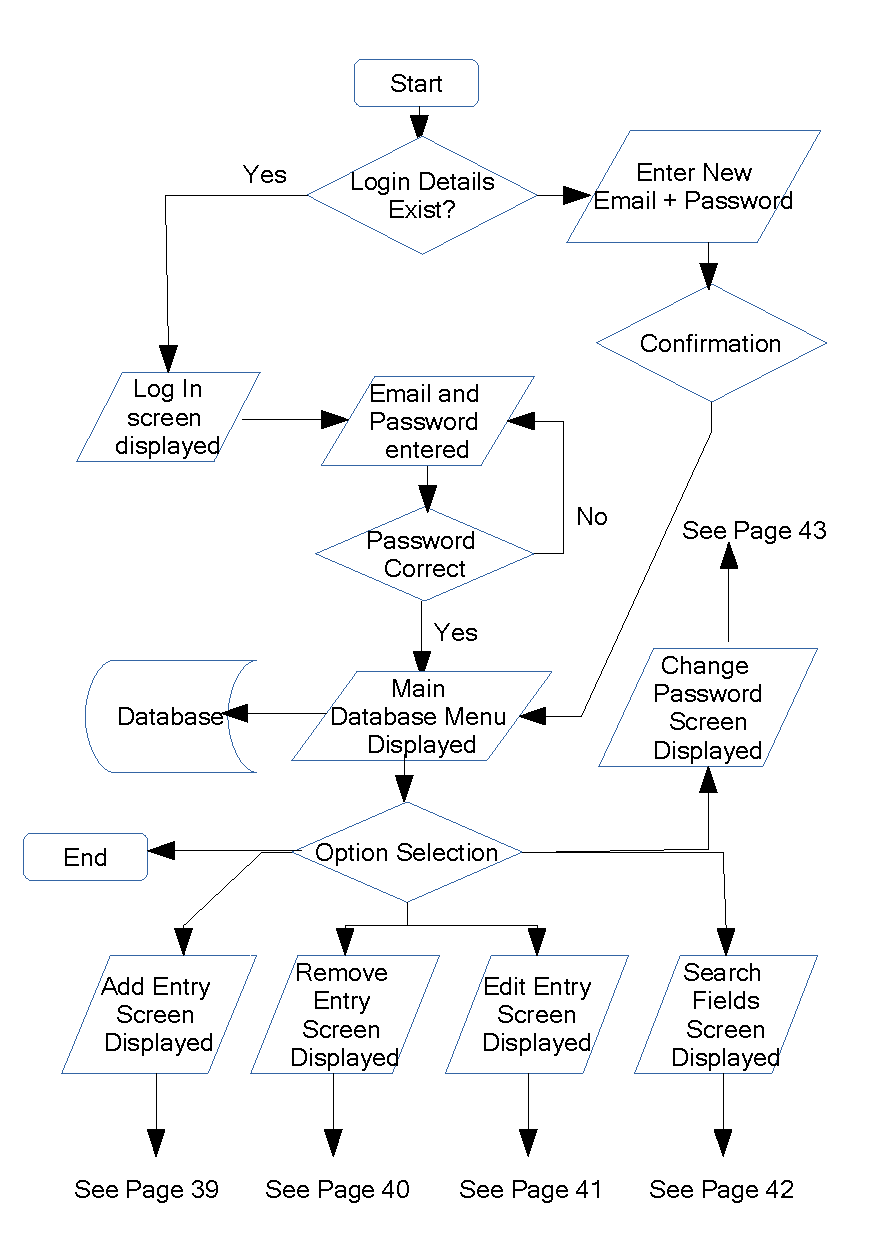
\includegraphics[width=\textwidth]{./Design/Flowcharts/Flowchart_1.pdf}
\end{figure}

\begin{figure}[H]
    \caption{Flowchart 2} \label{Flowchart_2.pdf}
    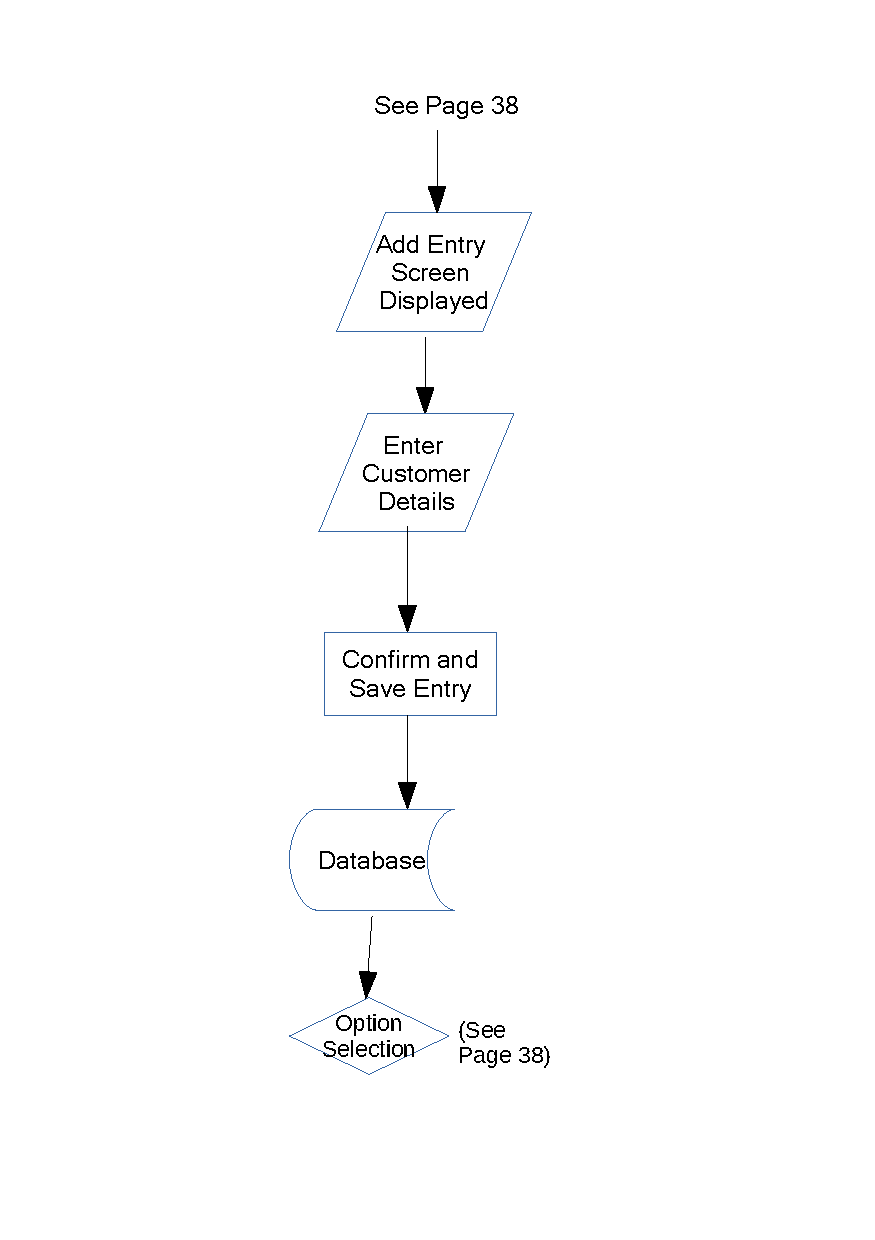
\includegraphics[width=\textwidth]{./Design/Flowcharts/Flowchart_2.pdf}
\end{figure}

\begin{figure}[H]
    \caption{Flowchart 3} \label{Flowchart_3.pdf}
    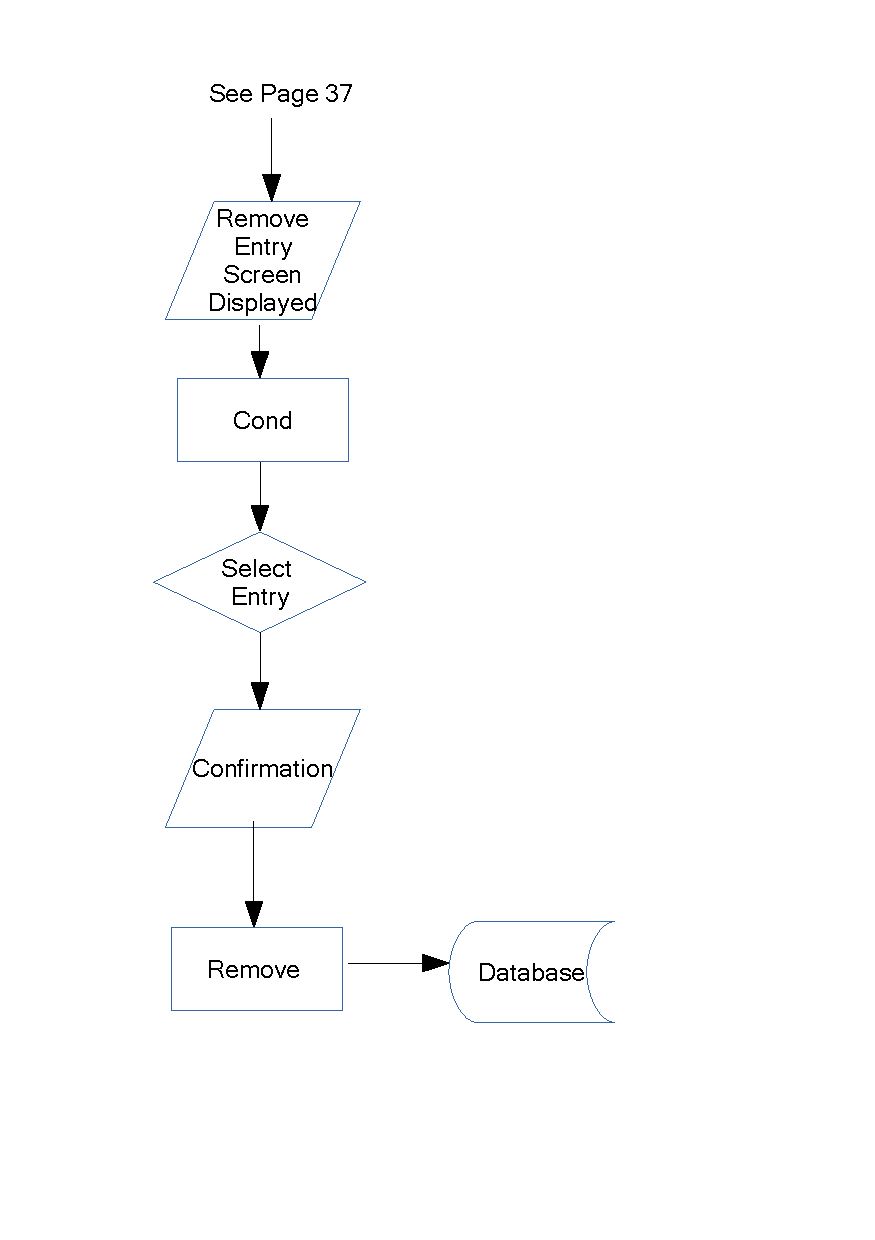
\includegraphics[width=\textwidth]{./Design/Flowcharts/Flowchart_3.pdf}
\end{figure}

\begin{figure}[H]
    \caption{Flowchart 4} \label{Flowchart_4.pdf}
    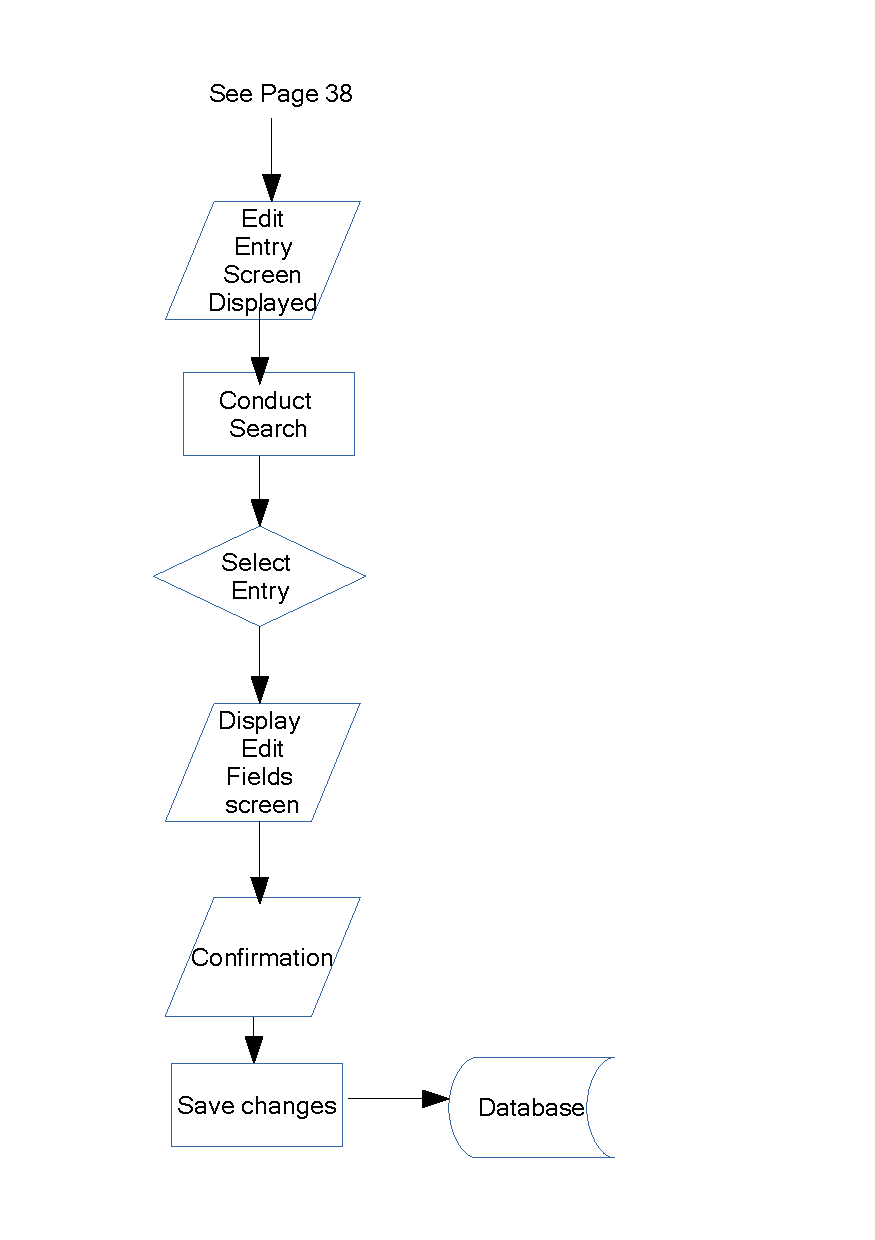
\includegraphics[width=\textwidth]{./Design/Flowcharts/Flowchart_4.pdf}
\end{figure}

\begin{figure}[H]
    \caption{Flowchart 5} \label{Flowchart_5.pdf}
    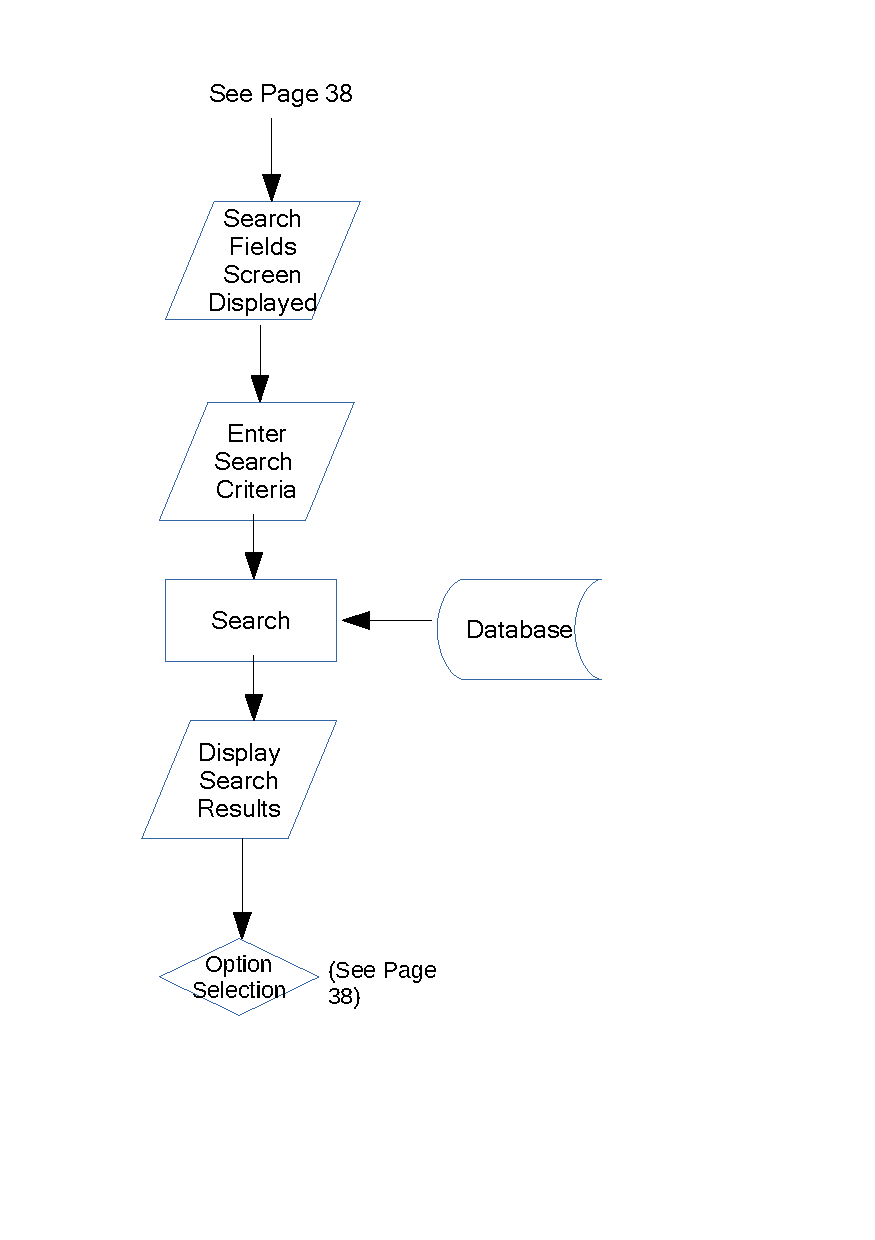
\includegraphics[width=\textwidth]{./Design/Flowcharts/Flowchart_5.pdf}
\end{figure}

\begin{figure}[H]
    \caption{Flowchart 6} \label{Flowchart_6.pdf}
    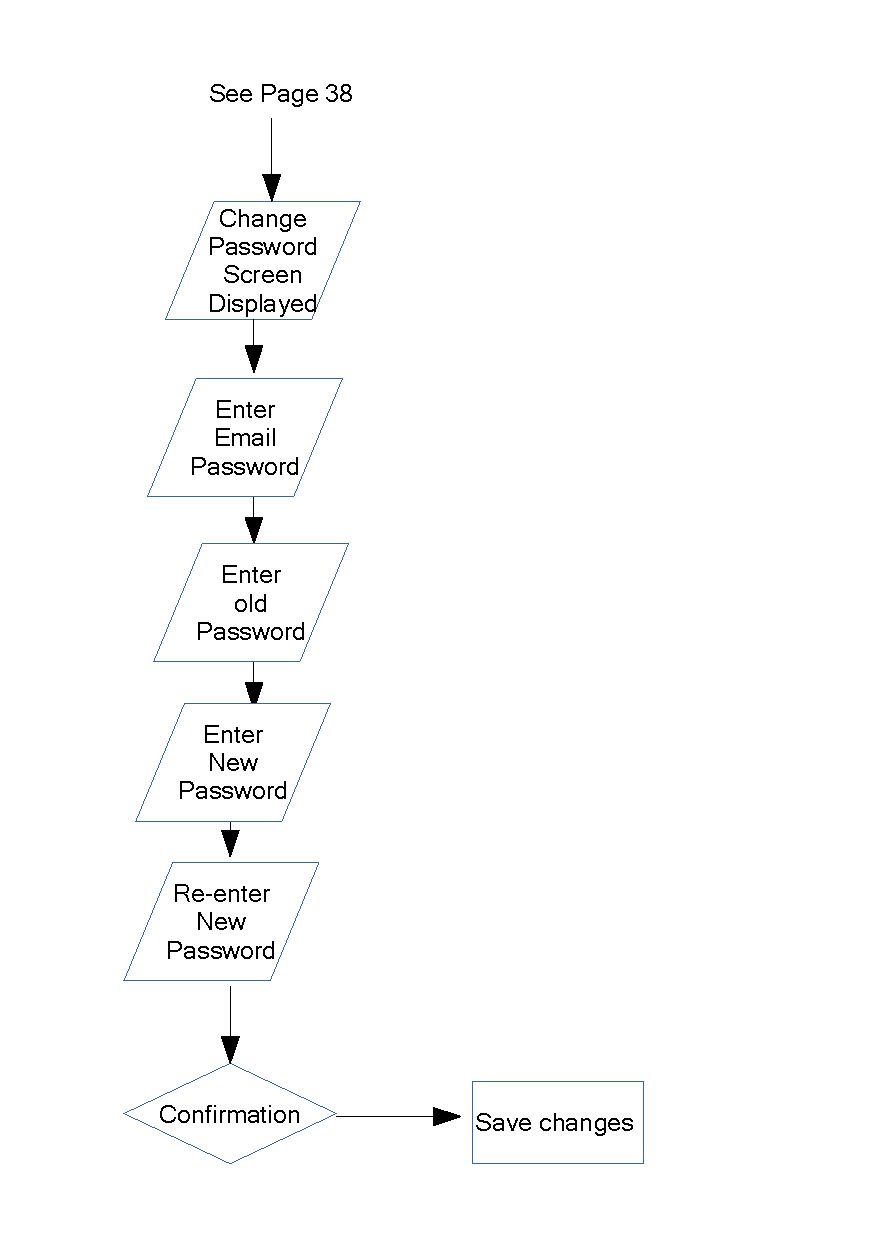
\includegraphics[width=\textwidth]{./Design/Flowcharts/Flowchart_6.pdf}
\end{figure}


\section{User Interface Designs}

\begin{figure}[H]
    \caption{Login Screen and Main Menu} \label{Login_Screen_and_Main_Menu.pdf}
    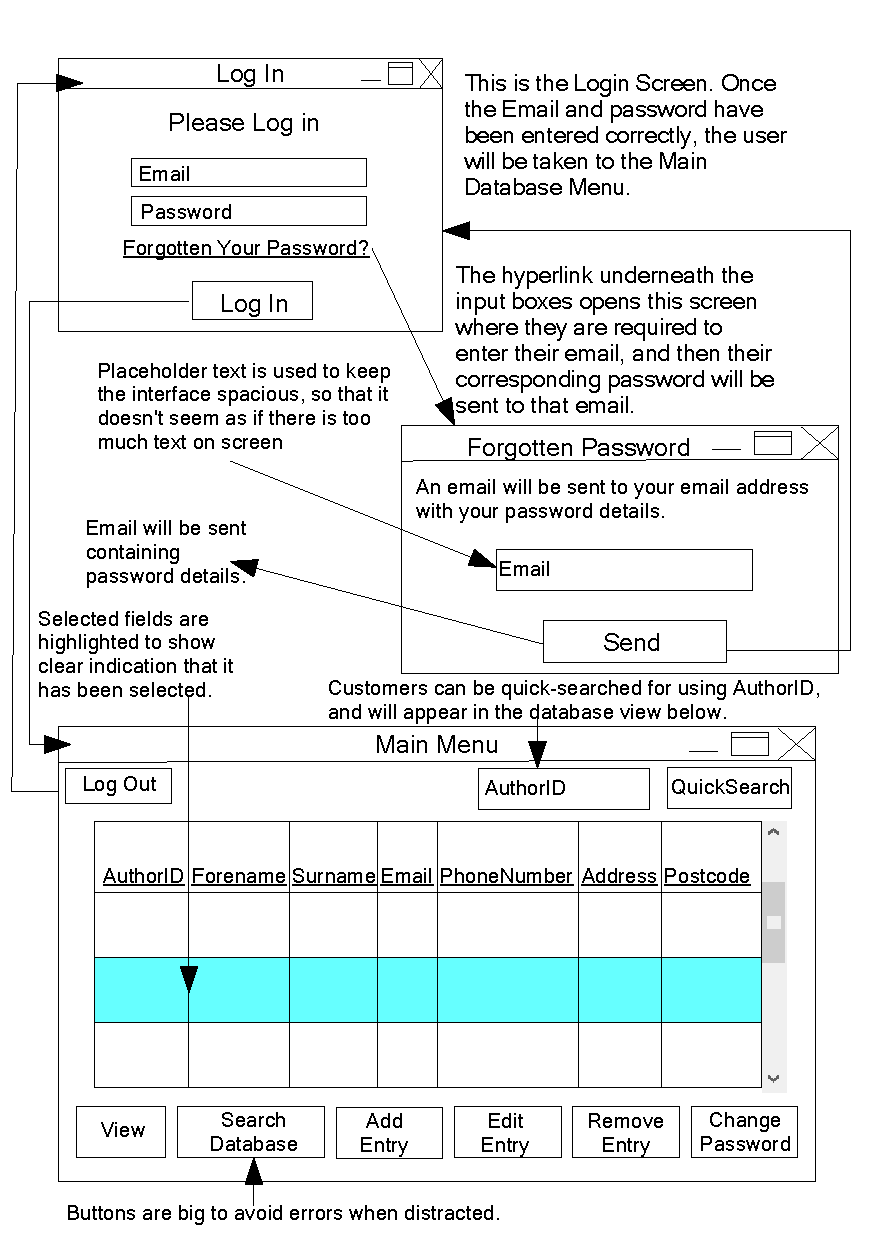
\includegraphics[width=\textwidth]{./Design/UserInterfaceDesign/Login_Screen_and_Main_Menu.pdf}
\end{figure}

\begin{figure}[H]
    \caption{View Menu and Royalties} \label{View_Menu_and_Royalties.pdf}
    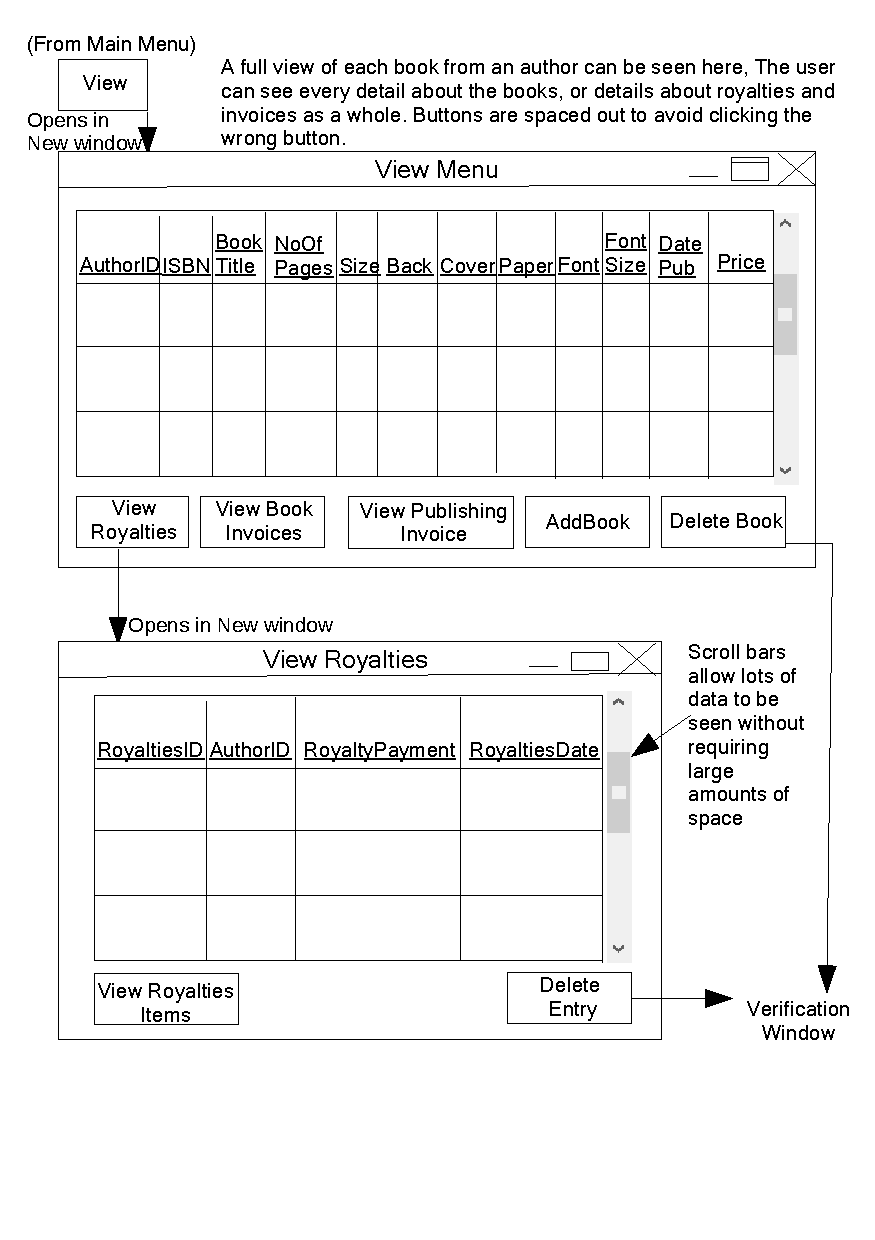
\includegraphics[width=\textwidth]{./Design/UserInterfaceDesign/View_Menu_and_Royalties.pdf}
\end{figure}

\begin{figure}[H]
    \caption{RoyaltiesItems and BookInvoice and Items} \label{RoyaltiesItems_and_BookInvoice_and_Items.pdf}
    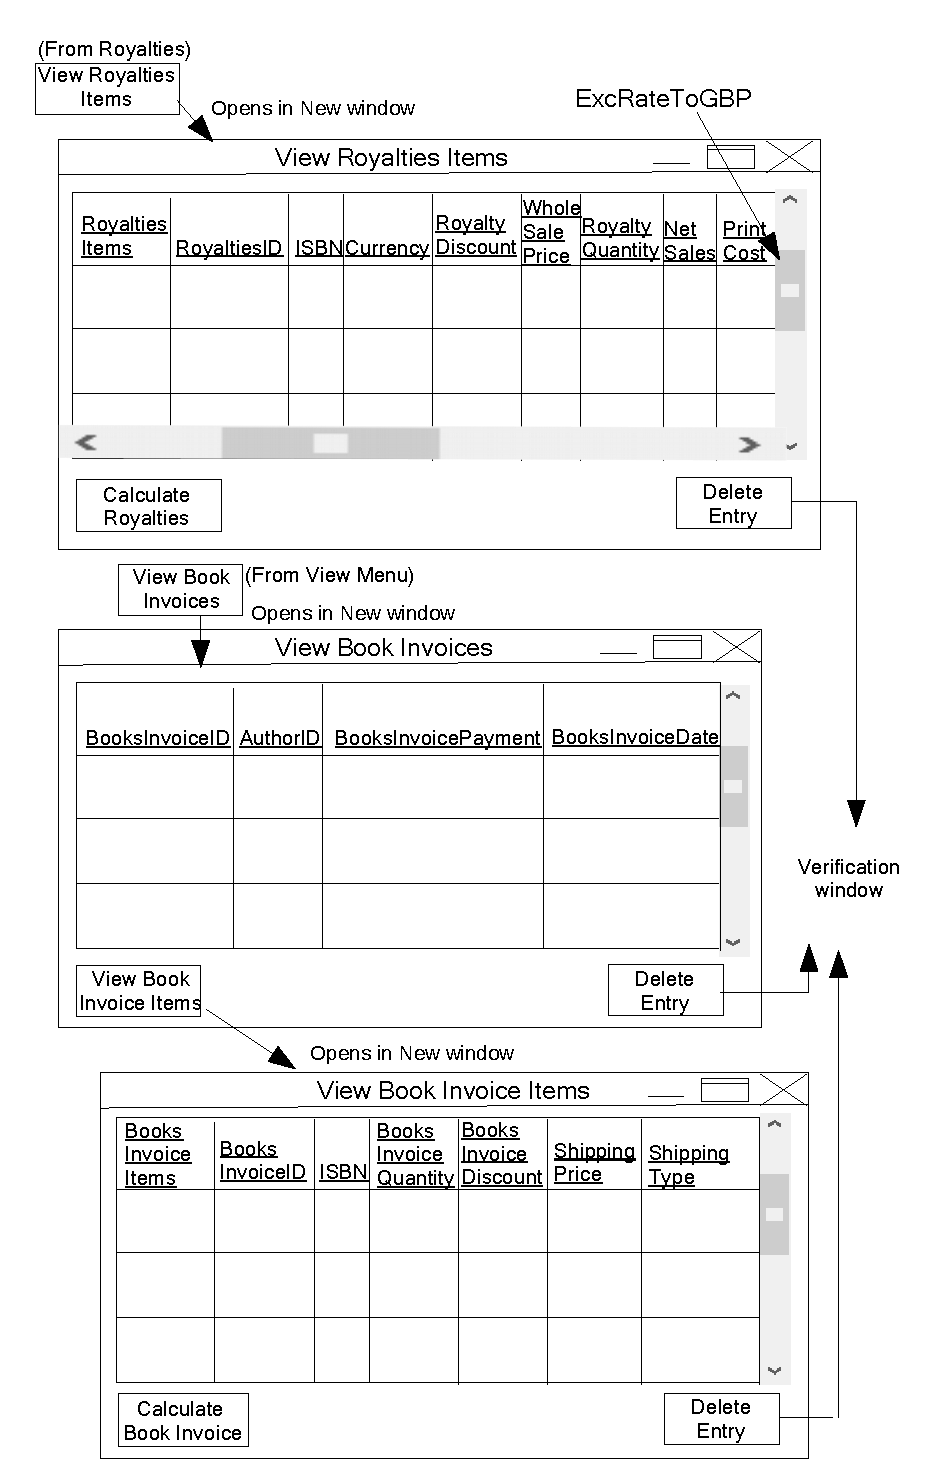
\includegraphics[width=\textwidth]{./Design/UserInterfaceDesign/RoyaltiesItems_and_BookInvoice_and_Items.pdf}
\end{figure}

\begin{figure}[H]
    \caption{Publishing Invoice and Adding Entries} \label{PubInvoice_and_Add_Entry.pdf}
    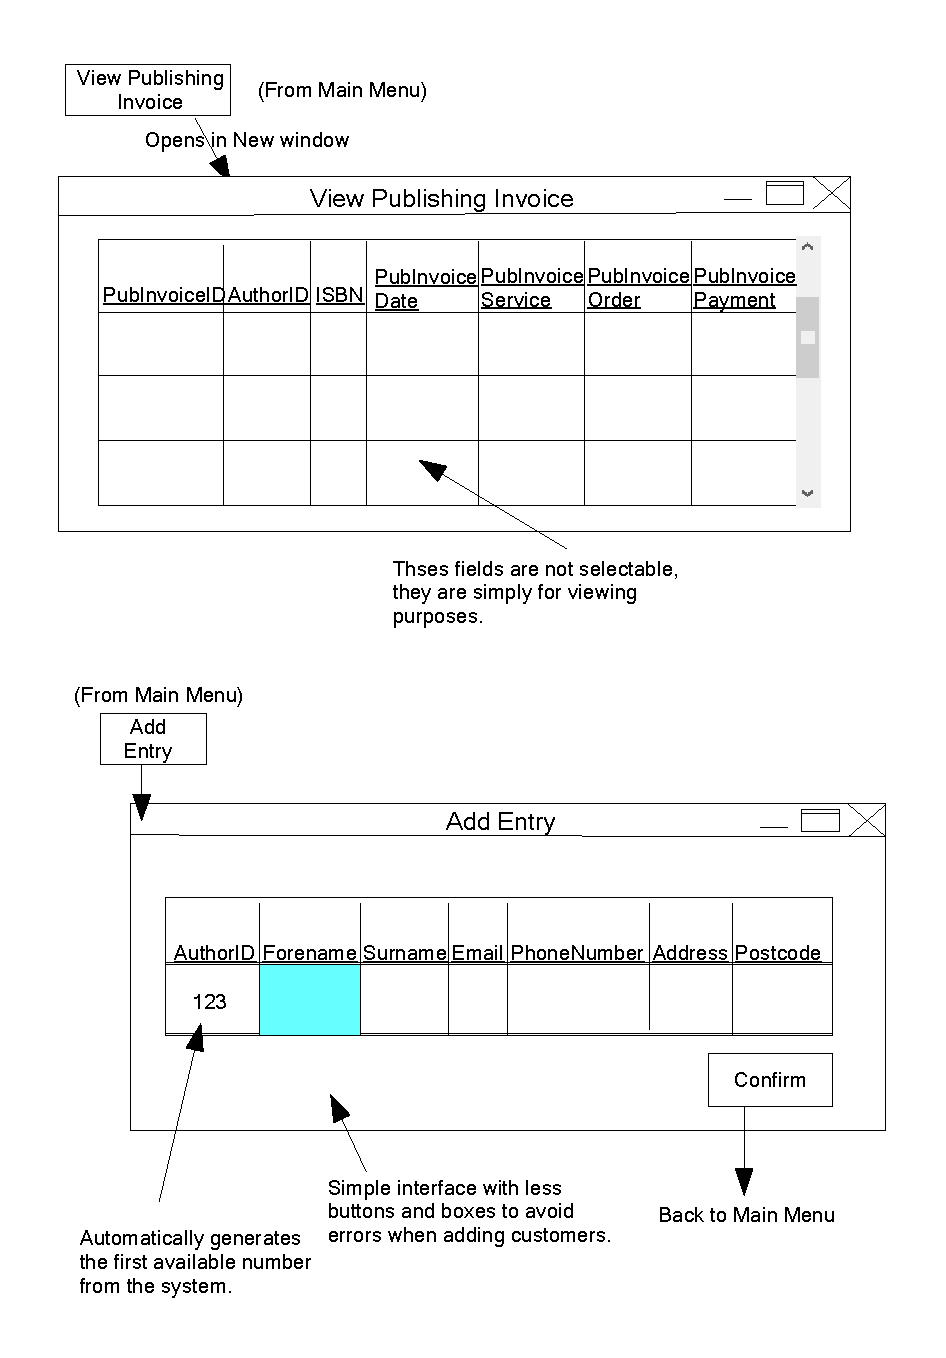
\includegraphics[width=\textwidth]{./Design/UserInterfaceDesign/PubInvoice_and_Add_Entry.pdf}
\end{figure}

\begin{figure}[H]
    \caption{Search} \label{Search.pdf}
    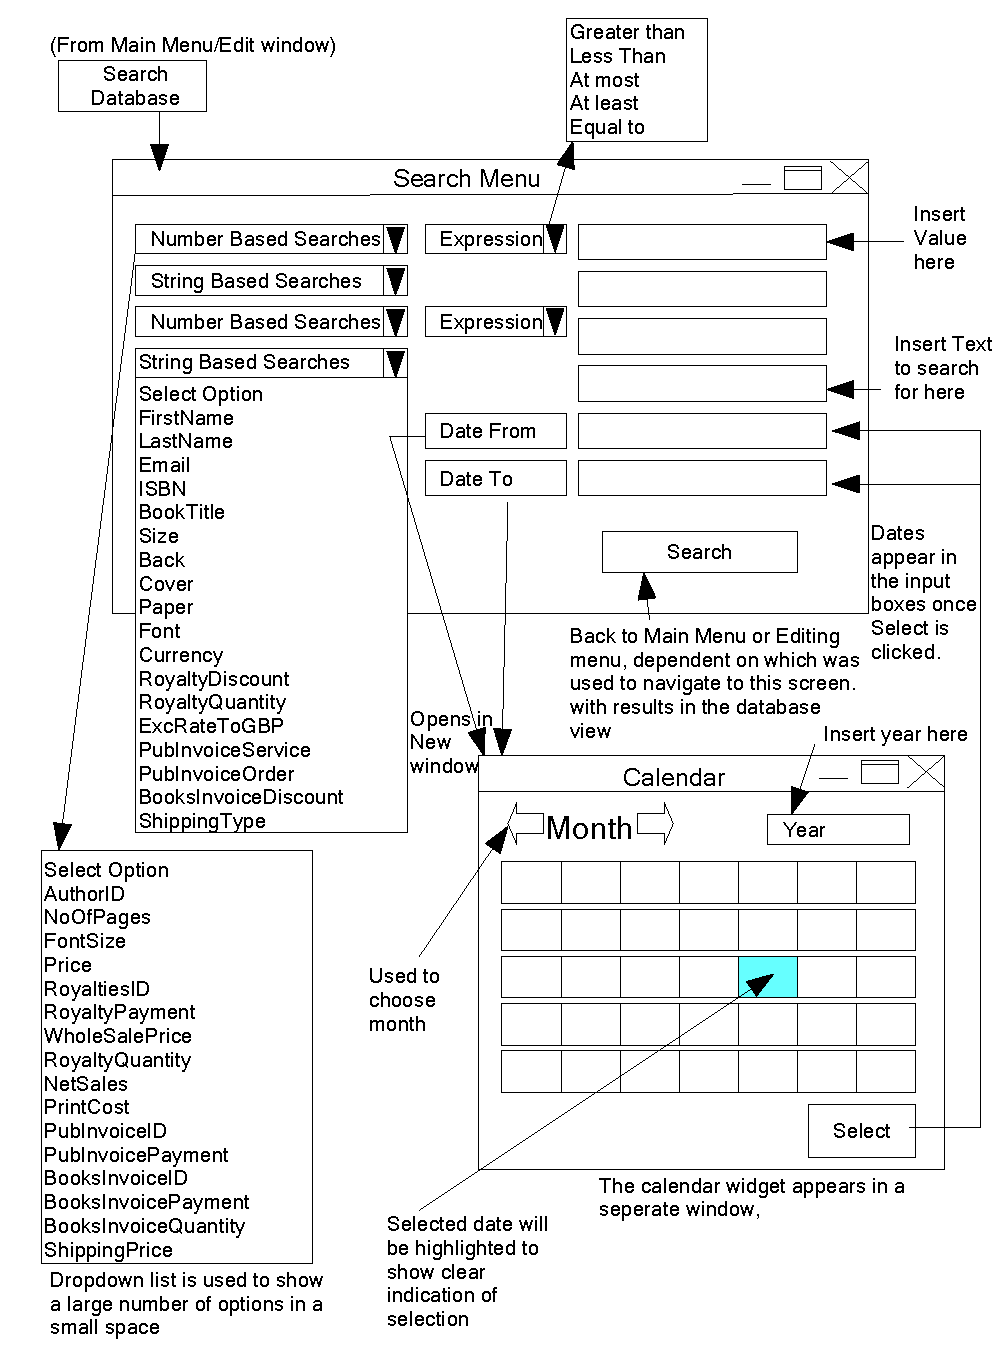
\includegraphics[width=\textwidth]{./Design/UserInterfaceDesign/Search.pdf}
\end{figure}

\begin{figure}[H]
    \caption{Editing Screens} \label{Editing_Screens.pdf}
    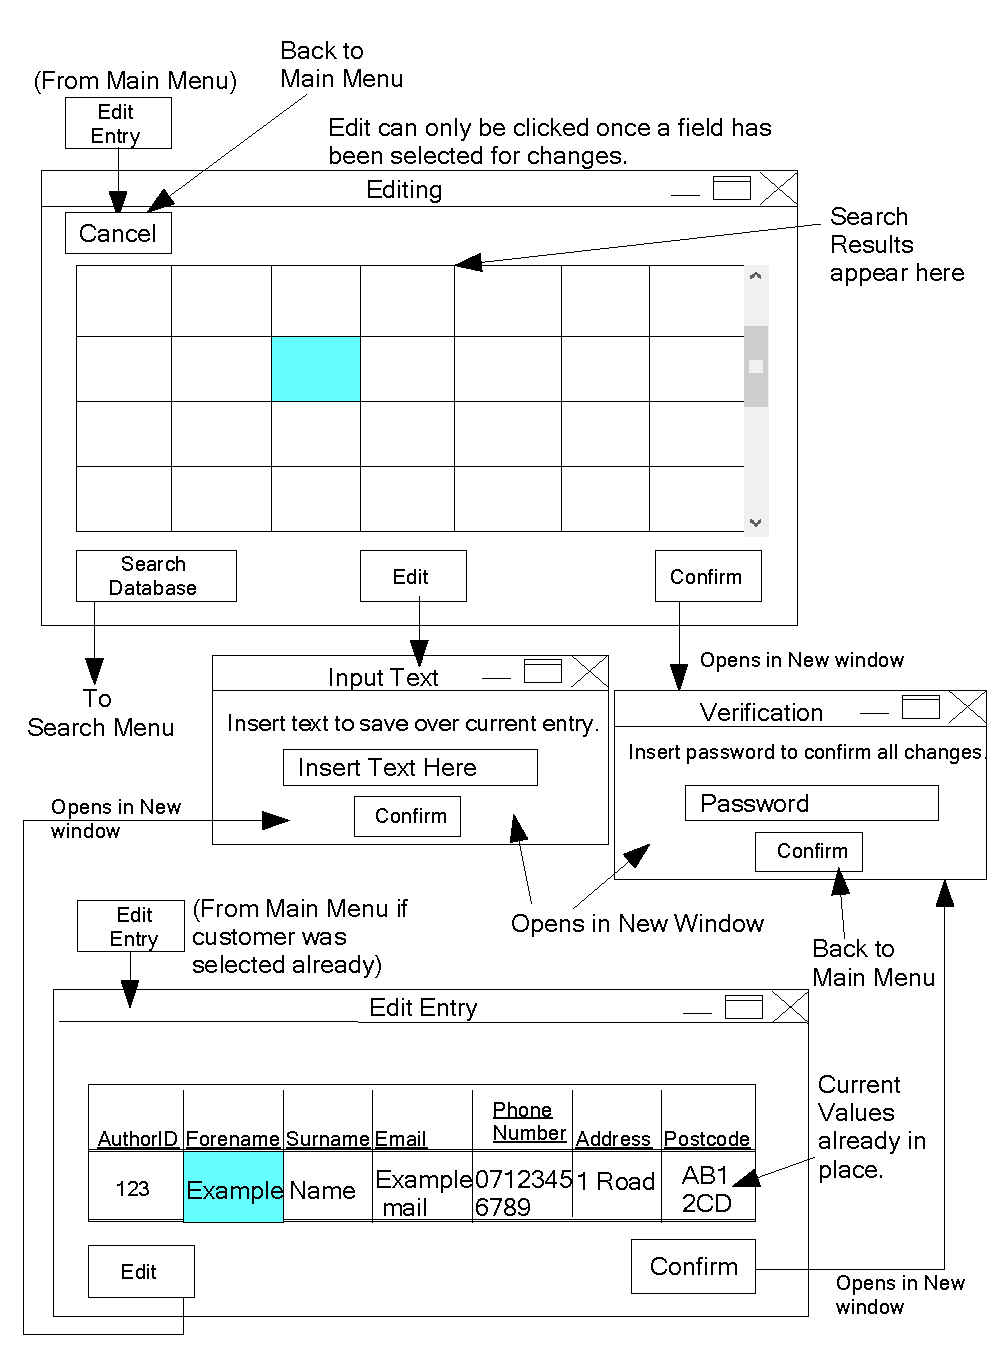
\includegraphics[width=\textwidth]{./Design/UserInterfaceDesign/Editing_Screens.pdf}
\end{figure}

\begin{figure}[H]
    \caption{Remove Entry and Change Password} \label{Remove_Entry_and_Change_Password.pdf}
    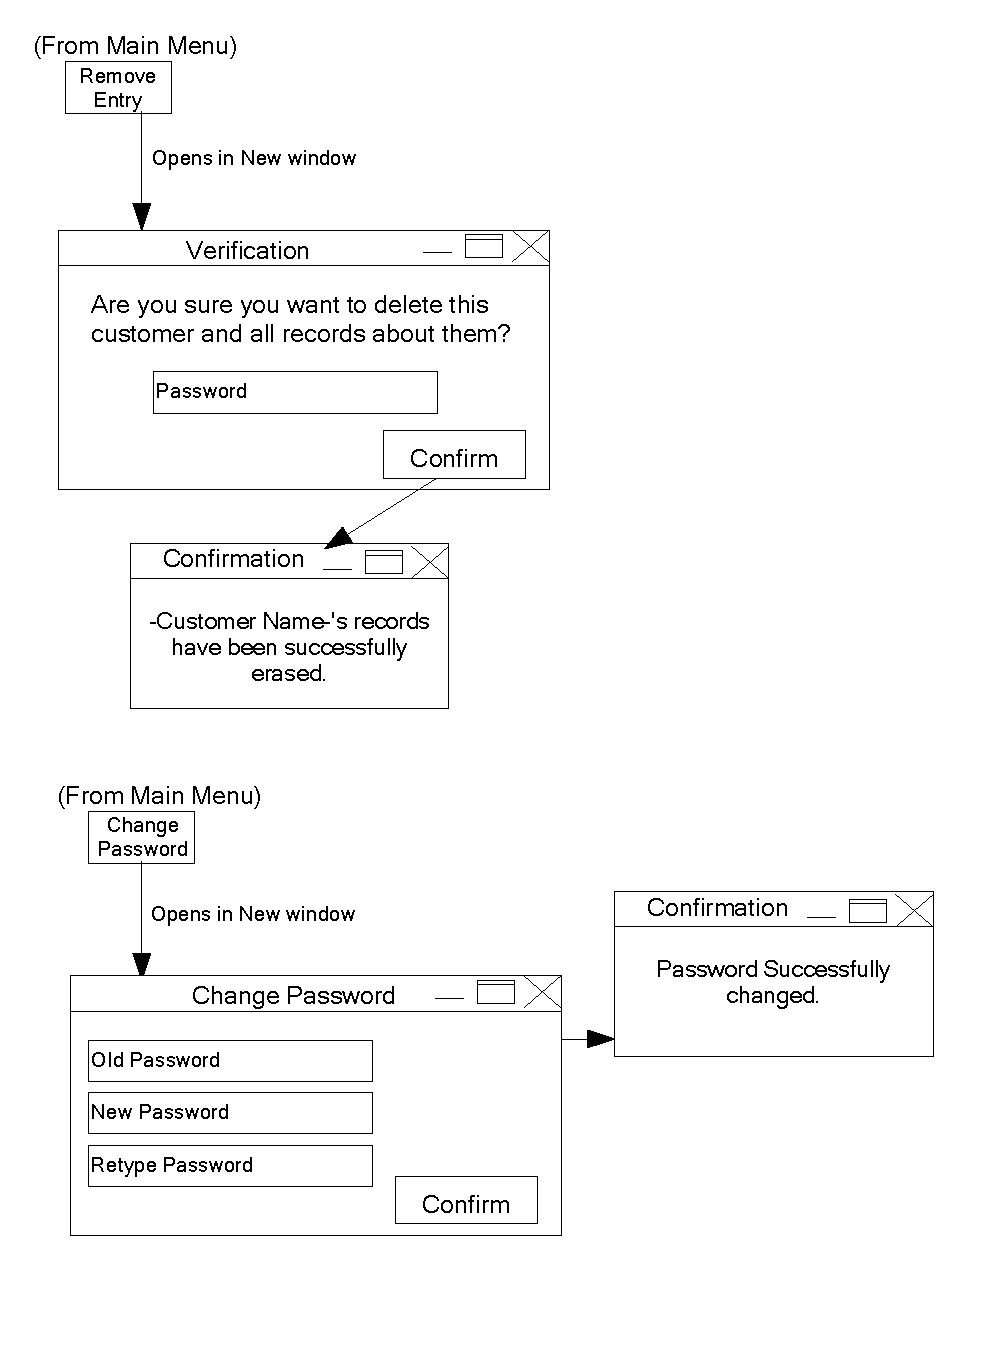
\includegraphics[width=\textwidth]{./Design/UserInterfaceDesign/Remove_Entry_and_Change_Password.pdf}
\end{figure}

\begin{figure}[H]
    \caption{Calculations} \label{Calculations.pdf}
    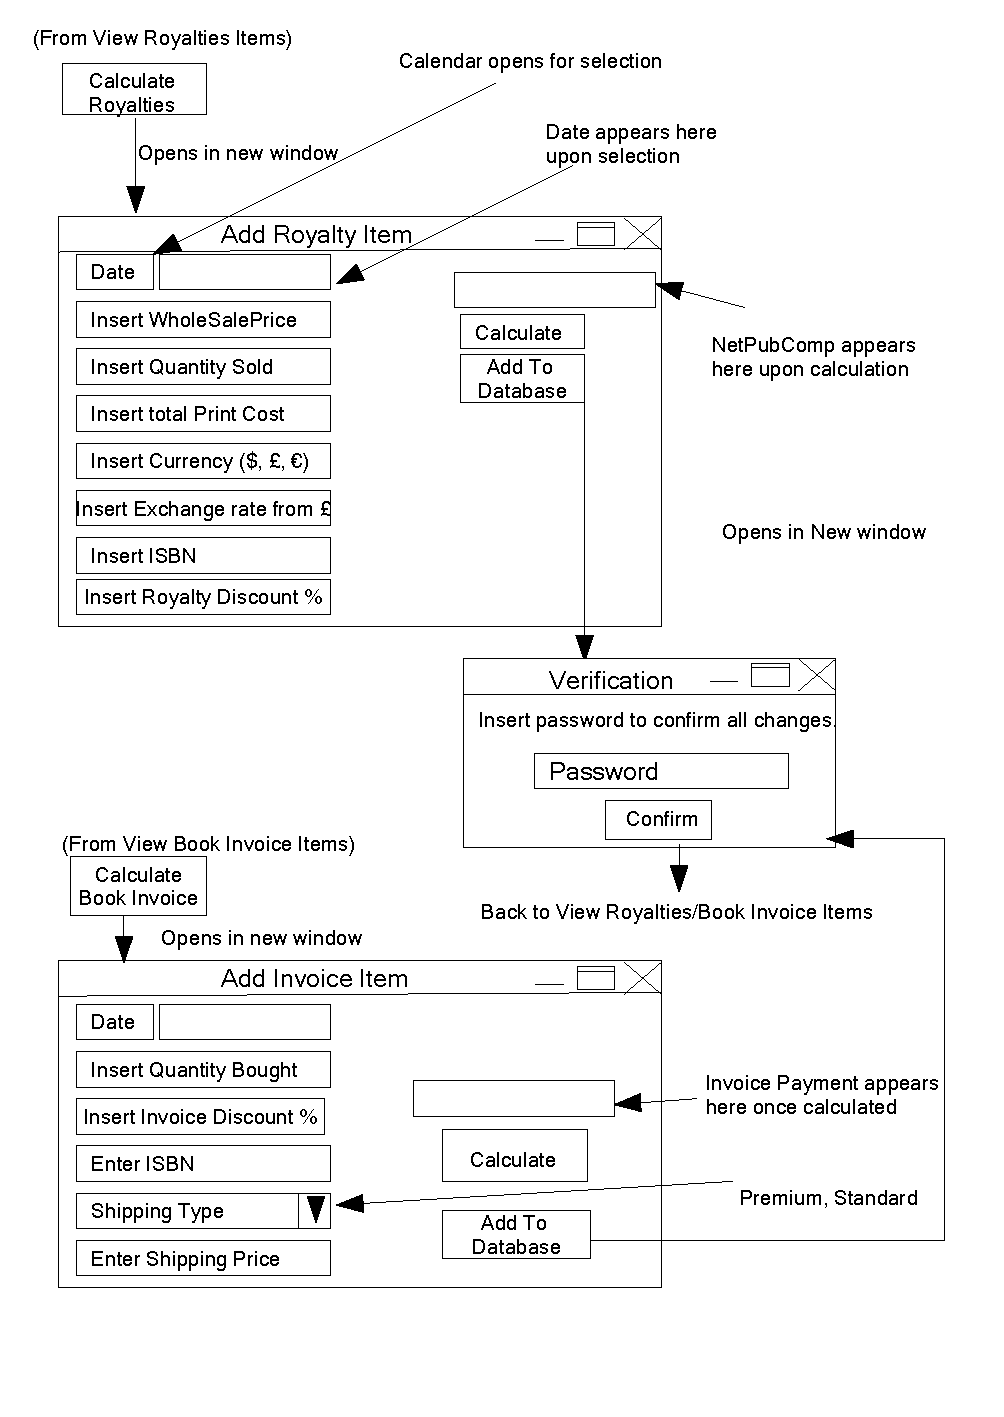
\includegraphics[width=\textwidth]{./Design/UserInterfaceDesign/Calculations.pdf}
\end{figure}

\begin{figure}[H]
    \caption{Adding Publishing Invoices} \label{AddPubInvoice.pdf}
    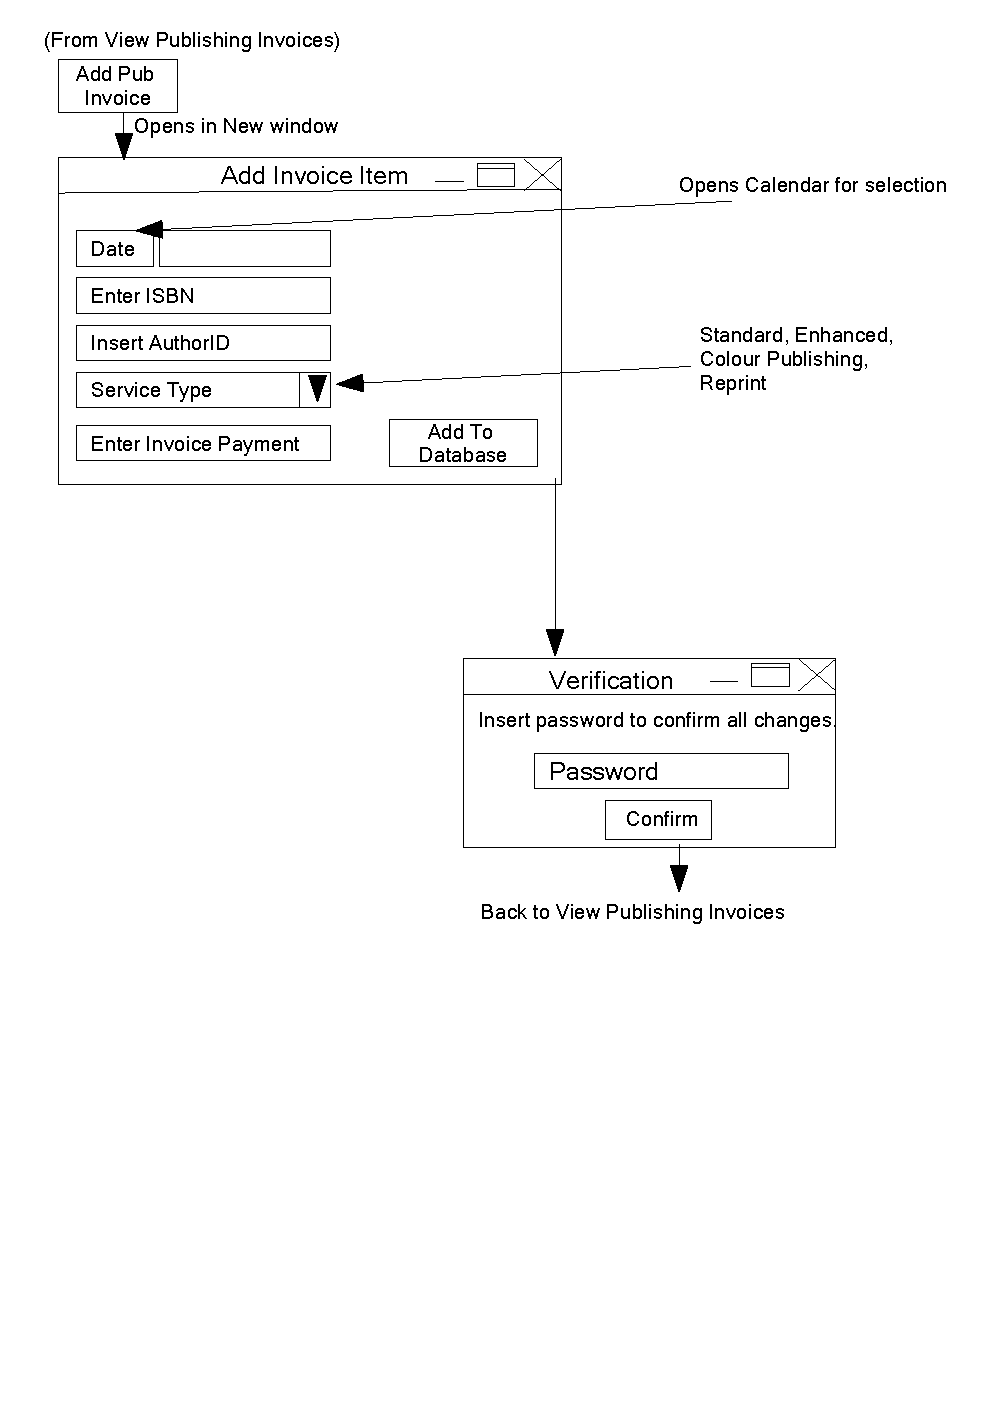
\includegraphics[width=\textwidth]{./Design/UserInterfaceDesign/AddPubInvoice.pdf}
\end{figure}

\begin{figure}[H]
    \caption{Add Book} \label{AddBook.pdf}
    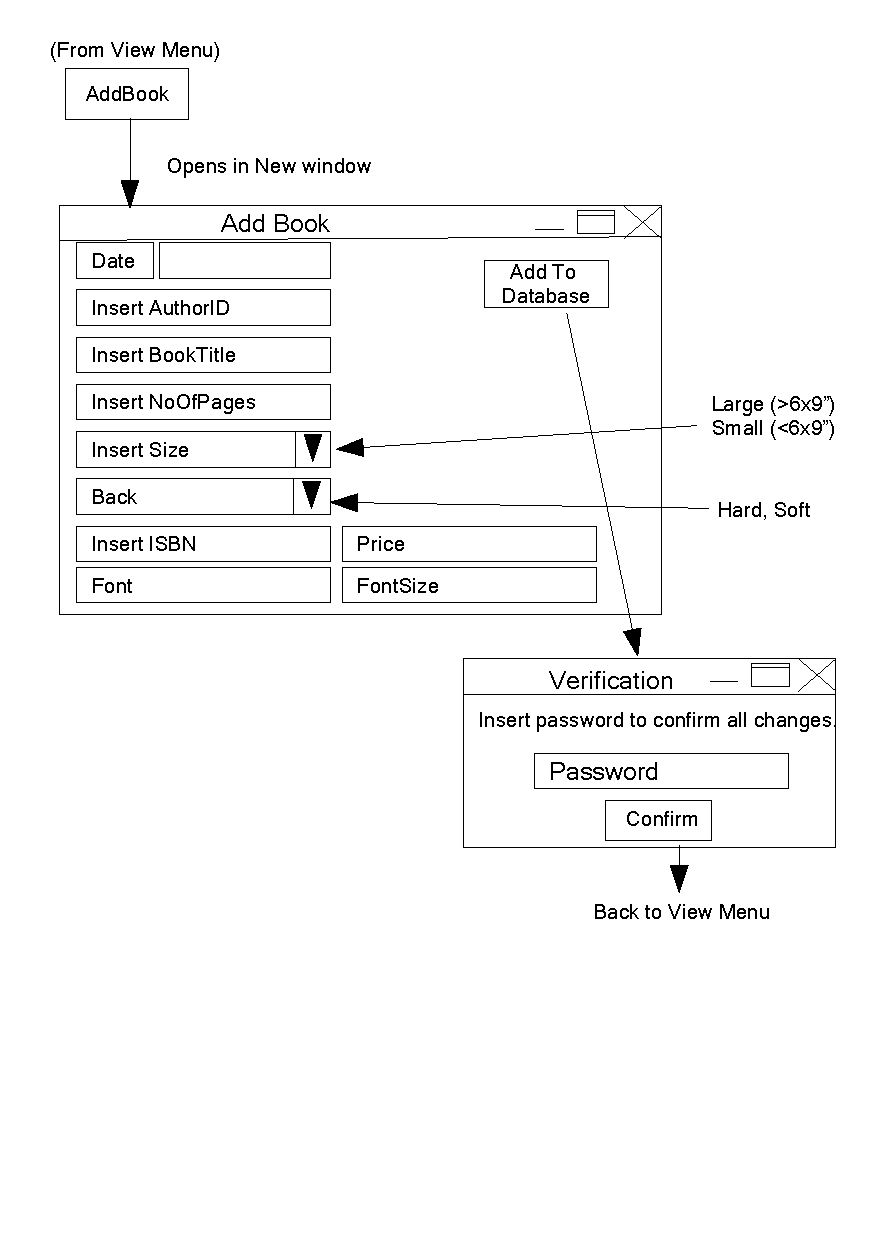
\includegraphics[width=\textwidth]{./Design/UserInterfaceDesign/AddBook.pdf}
\end{figure}

\section{Hardware Specification}

The system needs to be able to run on a laptop with a 1366 x 768, 16:9 aspect ratio screen which runs on Windows 8. This is imperative to the size of the application I will be creating because it must fit on the given screen size and can't be resizable. A mouse or touchpad will be used for navigational purposes, and for confirmation of entries. Also, a keyboard will be used for inputting information into fields for entering and editing information. All the data used by the program and its database will be held on a local hard drive, and a display is needed for the outputs of the program.

\section{Program Structure}

\subsection{Top-down design structure charts}

\subsection{Algorithms in pseudo-code for each data transformation process}

\begin{algorithm}[H]
    \caption{Add Customer Entry}
\begin{algorithmic}[1]

\Function{AddEntry}{CustomerTable}
Loop = 1
\SET{$GetNewAuthorID$}{$False$}
\SET{$ConfirmClicked$}{$False$}
NewAuthorID = 0

\While{$GetNewAuthorID = false$}

    NewAuthorID = loop
    Get AuthorID[loop] from CustomerTable

    \If{$NewAuthorID \ = \ AuthorID[loop]$}

        loop = loop +1

    \Else

        \SET{$GetNewAuthorID$}{$True$}

    \EndIf
\EndWhile

FirstName = null
LastName = null
Email = null
PhoneNumber = null
Address = null
Postcode = null

\While{$len(FirstName) <= 0$}

    INPUT FirstName

\EndWhile

\While{$len(LastName) <= 0$}

    INPUT LastName

\EndWhile

\While{$len(Email) <= 0$}

    INPUT Email

\EndWhile

\While{$len(PhoneNumber) <= 0$}

    INPUT PhoneNumber

\EndWhile

\While{$len(Address) <= 0$}

    INPUT Address

\EndWhile

\While{$len(Postcode) <= 0$}

    INPUT Postcode

\EndWhile

\If{$ConfirmClicked \ == \ True$}

    CONNECT to Customer Database

\EndIf
\EndFunction
\end{algorithmic}
\end{algorithm}

\begin{algorithm}[H]
    \caption{Add and Calculate Royalty Items}
\begin{algorithmic}[1]

\Function{AddRoyaltyItem}{}

\SET{$CalculateClicked$}{$False$}
\SET{$AddToDatabaseClicked$}{$False$}

Date = null
WholeSalePrice = null
QuantitySold = null
PrintCost = null
Currency = null
ExcRateFromGBP = null
ISBN = null
RoyaltyDiscount = null

\While{$len(Date) <= 0$}

    INPUT Date

\EndWhile

\While{$len(WholeSalePrice) <= 0$}

    INPUT WholeSalePrice

\EndWhile

\While{$len(QuantitySold) <= 0$}

    INPUT LastName

\EndWhile

\While{$len(PrintCost) <= 0$}

    INPUT PrintCost

\EndWhile

\While{$len(Currency) <= 0$}

    INPUT Currency

\EndWhile

\If{$Currency \ <> \ £$}

    \While{$len(ExcRatefromGBP) <= 0$}

        INPUT ExcRateFromGBP

    \EndWhile
\EndIf

\While{$len(ISBN) <= 0$}

    INPUT ISBN

\EndWhile

\While{$len(RoyaltyDiscount) <= 0$}

    INPUT RoyaltyDiscount
    \If{$RoyaltyDiscount \ > \ 100$}

        RoyaltyDiscount = null

    \EndIf

    \If{$RoyaltyDiscount \ < \ 0$}

        RoyaltyDiscount = null

    \EndIf
\EndWhile

\If{$CalculateClicked \ == \ True$}

    NetSales = WholeSalePrice * RoyaltyQuantity
    NetPubComp = NetSales - PrintCost
    OUTPUT NetPubComp

\EndIf

\If{$AddToDatabaseClicked \ == \ True$}
    
    CONNECT to RoyaltyItems Database
    
\EndIf

\EndFunction
\end{algorithmic}
\end{algorithm}


\begin{algorithm}[H]
    \caption{Add and Calculate Invoice Items}
\begin{algorithmic}[1]

\Function{AddInvoiceItem}{BookTable}

\SET{$CalculateClicked$}{$False$}
\SET{$AddToDatabaseClicked$}{$False$}

Date = null
QuantityBought = null
InvoiceDiscount = null
ShippingType= null
ShippingPrice= null
ISBN = null


\While{$len(Date) <= 0$}

    INPUT Date

\EndWhile

\While{$len(QuantityBought) <= 0$}

    INPUT QuantityBought

\EndWhile

\While{$len(InvoiceDiscount) <= 0$}

    INPUT InvoiceDiscount

\EndWhile

\While{$len(ISBN) <= 0$}

    INPUT ISBN

\EndWhile

\While{$len(ShippingType) <= 0$}

    INPUT ShippingType

\EndWhile

\While{$len(ShippingPrice) <= 0$}

    INPUT ShippingPrice

\EndWhile

\If{$CalculateClicked \ == \ True$}

    InvoicePayment = QuantityBought * Price * InvoiceDiscount + Shipping Price
    OUTPUT InvoicePayment

\EndIf

\If{$AddToDatabaseClicked \ == \ True$}
    
    CONNECT to Invoice Database
    
\EndIf

\EndFunction
\end{algorithmic}
\end{algorithm}

\begin{algorithm}[H]
    \caption{Add Book}
\begin{algorithmic}[1]

\Function{AddInvoiceItem}{CustomerTable}

\SET{$AddToDatabaseClicked$}{$False$}

DatePublished = null
ISBN = null
AuthorID = null
BookTitle = null
NoOfPages = null
Size = null
Back = null
Cover = null
Paper = null
Font = null
FontSize = null
Price = null

\While{$len(DatePublished) <= 0$}

    INPUT DatePublished

\EndWhile

\While{$len(ISBN) <= 0$}

    INPUT ISBN

\EndWhile

\While{$len(BookTitle) <= 0$}

    INPUT BookTitle

\EndWhile

\While{$len(Size) <= 0$}

    INPUT Size

\EndWhile

\While{$len(BackType) <= 0$}

    INPUT BackType

\EndWhile

\While{$len(NoOfPages) <= 0$}

    INPUT NoOfPages

\EndWhile

\While{$len(Paper) <= 0$}

    INPUT Paper

\EndWhile

\While{$len(Font) <= 0$}

    INPUT Font

\EndWhile

\While{$len(FontSize) <= 0$}

    INPUT FontSize

\EndWhile

\While{$len(Price) <= 0$}

    INPUT Price

\EndWhile

\If{$AddToDatabaseClicked \ == \ True$}
    
    CONNECT to Book Database
    
\EndIf

\EndFunction
\end{algorithmic}
\end{algorithm}

\begin{algorithm}[H]
    \caption{Add and Publishing Invoice}
\begin{algorithmic}[1]

\Function{AddInvoiceItem}{BookTable, CustomerTable}

\SET{$AddToDatabaseClicked$}{$False$}

Date = null
AuthorID = null
ServiceType = null
InvoicePayment= null
ISBN = null

\While{$len(Date) <= 0$}

    INPUT Date

\EndWhile

\While{$len(AuthorID) <= 0$}

    INPUT AuthorID

\EndWhile

\While{$len(InvoicePayment) <= 0$}

    INPUT InvoicePayment

\EndWhile

\While{$len(ISBN) <= 0$}

    INPUT ISBN

\EndWhile

\While{$len(ServiceType) <= 0$}

    INPUT ServiceType

\EndWhile

\If{$AddToDatabaseClicked \ == \ True$}
    
    CONNECT to PubInvoice Database
    
\EndIf

\EndFunction
\end{algorithmic}
\end{algorithm}



\subsection{Object Diagrams}

\subsection{Class Definitions}

\section{Prototyping}

It will be helpful to create a prototype of the main menu to make sure that different windows can be navigated through without any difficulty. This would give me a good idea of the flow of control between interfaces. Also, I plan to prototype a log in screen, because this would help me identify the difficulties involved in moving to and from the main menu and log in screen.

Furthermore, I plan to prototype the adding, editing and removal of data to and from the database. I am going to prototype this in order to make sure that data can be successfully added, edited and removed to and from the database so that it can be confirmed that this can be conducted upon creation of the program.

I have already prototyped the calendar interface used for inputting the date in a box. This is just a prototype of the basic interface, which is for selecting a date and placing it in the text box. It can switch between months with a dropdown list, or using the arrows and also years.

\begin{figure}[H]
    \caption{Calendar Interface} \label{Calendar_1.pdf}
    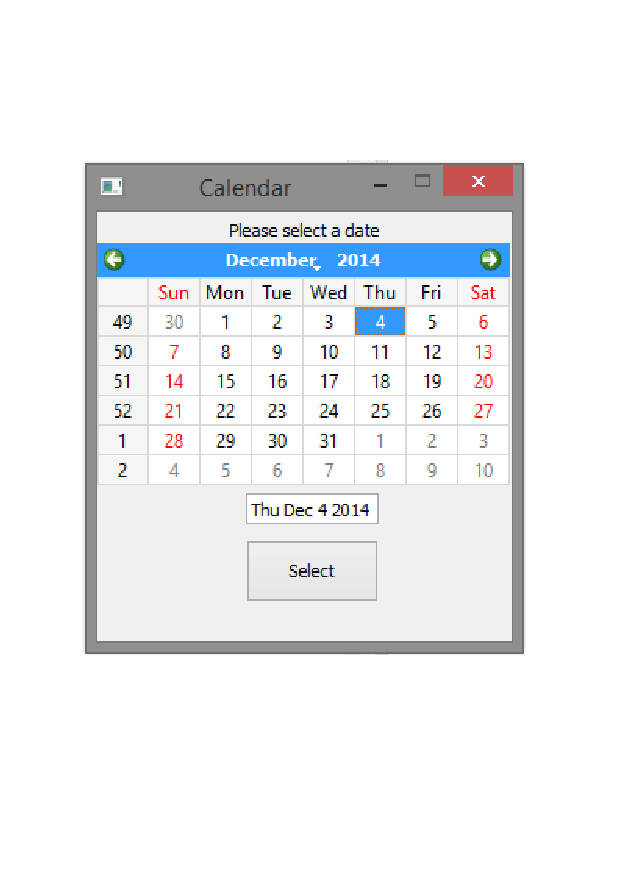
\includegraphics[width=\textwidth]{./Design/Calendar_1.pdf}
\end{figure}

\begin{figure}[H]
    \caption{Calendar - Date Selection} \label{Calendar_2.pdf}
    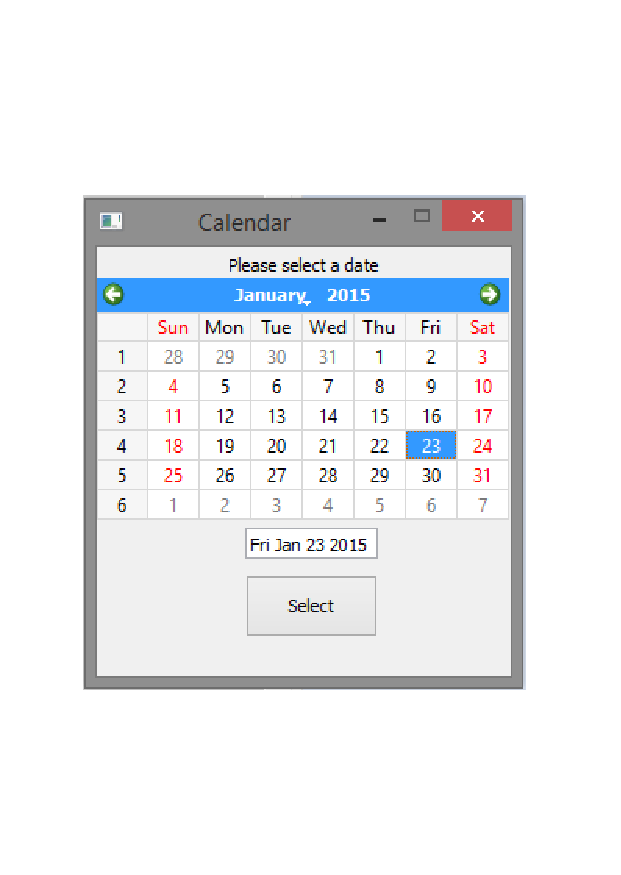
\includegraphics[width=\textwidth]{./Design/Calendar_2.pdf}
\end{figure}

\section{Definition of Data Requirements}

\subsection{Identification of all data input items}

\subsection{Identification of all data output items}

\subsection{Explanation of how data output items are generated}

\subsection{Data Dictionary}

There have been some changes to my data dictionary as a number of elements have been identified that need to be added to the system.

\begin{center}
\begin{tabular}{|p{2cm}|p{1cm}|p{2.5cm}|p{1.5cm}|p{3cm}|}
    \hline
    \textbf{Name} & \textbf{Data Type} & \textbf{Length} & \textbf{Validation} & \textbf{Example Data} \\ \hline
    FirstName & String & 2-20 Characters & Length & Jo  \\ \hline
    LastName & String & 2-20 Characters & Length & Williamson  \\ \hline
    Email & String & 7-30 Characters & Length & mail@example.com  \\ \hline
    PhoneNumber & String & 9-15 Characters & Format & 07123456789  \\ \hline
    Address & String & 5-64 Characters & Length & Example Road  \\ \hline
    Postcode & String & 7 Characters & Format & AB1 2CD  \\ \hline
    AuthorID & Integer & 1-255 & Range & 17  \\ \hline
    ISBN & String & 13 Characters & Length & 9780007525492 \\ \hline
    BookTitle & String & 1-127 Characters & Length & The Hobbit  \\ \hline
    NoOfPages & Integer & 1-1023 & Range & 395  \\ \hline
    Size & String & 5 & Existence & Large \\ \hline
    Back & String & 8 or 9 Characters& Existence & Paperback  \\ \hline
    Cover & String & 3 or 5 Characters & Existence & Gloss \\ \hline
    Paper & String & 11 Characters & Existence & White Paper\\ \hline
    Font & String & 1-64 Characters & Length & Arial  \\ \hline
    FontSize & Real & 8-64 & Numbers only & 12.5  \\ \hline
    DatePublished & Date & dd/mm/yyyy & Range & 23/10/2014 \\ \hline
    Price & Real & 0.01-63.00 & Numbers only & £12.99 \\ \hline
    RoyaltiesID & Integer & 1-255 & Numbers only & 123 \\ \hline
    RoyaltiesItems & Integer & 1-511 & Numbers only & 12 \\ \hline
    Currency & String & 1 Character & Pound, Dollar or Euro sign & £ \\ \hline
    RoyaltyPayment & Real & 1-32767 & Numbers only & 489.92 \\ \hline
    RoyaltiesDate & Date & dd/mm/yyyy & Range & 03/12/2014 \\ \hline
    RoyaltyDiscount & Real & 0-100 & Numbers only & 40 \\ \hline
    WholeSalePrice & Real & 0.01-63.00 & Numbers only & 7.99 \\ \hline
    RoyaltyQuantity & Integer & 1- 2047 & Numbers only & 192 \\ \hline
    NetSales & Real & 0.01-32767.00 & Numbers only & 900.00 \\ \hline
    PrintCost & Real & 0.01-32767.00 & Numbers only & 800.00 \\ \hline
    ExcRateFromGBP & Real & 0-1027 & Numbers only & 1.67 \\ \hline
    PubInvoiceID & Integer & 1-511 & Numbers only & 123 \\ \hline
    PubInvoiceDate & Date & dd/mm/yyy & Range & 23/05/2014 \\ \hline
    PubInvoiceService & String & 1-127 Characters & Length & Standard \\ \hline
    PubInvoicePayment & Real & 0.01-32767.00 & Numbers only & 700.00 \\ \hline
    BooksInvoiceID & Integer & 1-255 & Numbers only & 99 \\ \hline
    BooksInvoiceItems & Integer & 1-255 & Numbers only & 2 \\ \hline
    BooksInvoicePayment & Real & 0.01-32767.00 & Numbers only & 600.00 \\ \hline
    BooksInvoiceTotal & Real & 0.01-32767.00 & Numbers only & 500.00 \\ \hline
    BooksInvoiceDate & Date & dd/mm/yyyy & Range & 01/01/2014 \\ \hline
    BooksInvoiceDiscount & Real & 0-100 & Numbers only & 50 \\ \hline
    BooksInvoiceQuantity & Integer & 1-2047 & Numbers only & 777 \\ \hline
    Shipping Type & String & 7-8 Characters & Range & Premium \\ \hline
    Shipping Price & Real & 0.01-64.00 & Numbers only & 25.00 \\ \hline
    \hline
\end{tabular}
\end{center}

\subsection{Identification of appropriate storage media}


\newpage

\section{Database Design}

\subsection{Normalisation}
 
\subsubsection{ER Diagrams}


\begin{figure}[H]
    \caption{ER Diagram} \label{ER_Diagram.pdf}
    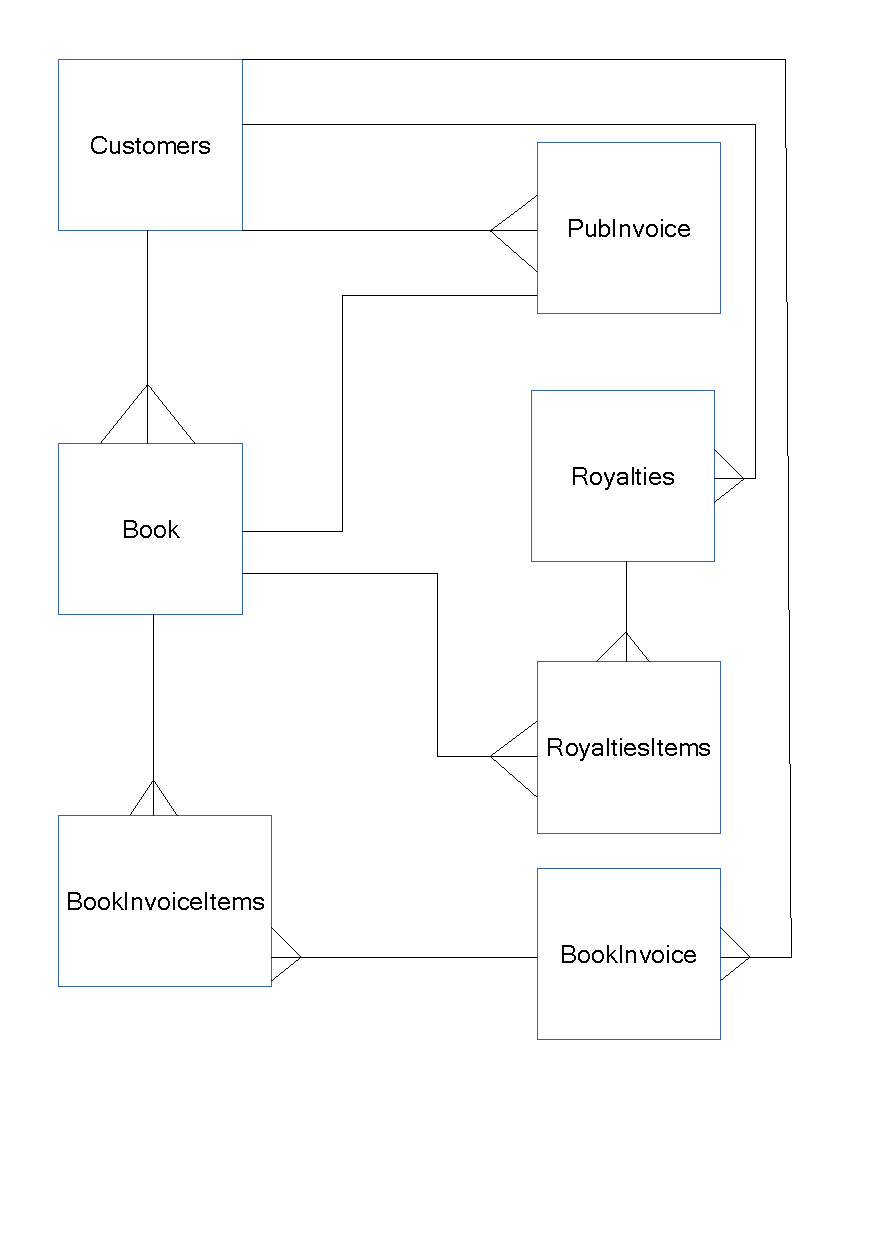
\includegraphics[width=\textwidth]{./Design/ER_Diagram.pdf}
\end{figure}


\subsubsection{Entity Descriptions}

Customer(\underline{Author ID}, FirstName, LastName, Email, Address, Postcode, Phone Number)

Invoice(\underline{InvoicePayment}, \underline{InvoiceDate}, \emph{ISBN}, \emph{AuthorID}, InvoiceQuantity, InvoiceDiscount, ShippingPrice, ShippingType)

Royalties(\underline{RoyaltyPayment}, \underline{RoyaltiesDate}, \emph{ISBN}, \emph{AuthorID}, RoyaltyDiscount, WholeSalePrice, RoyaltyQuantity, NetSales, PrintCost)

Book(\underline{ISBN}, \emph{AuthorID}, Book Title, NoOfPages, Size, Cover, Paper, Back, Paper, Font, FontSize, DatePublished, Price)

\subsubsection{UNF to 3NF}

Key:

\textbf{Bold Font} = Primary Key

\emph{Italics} = Foreign Key

Each Column represents a new group.

\newpage
First of all, I have started with the data in its unnormalised form.

\begin{tabular}{|p{3.5cm}|}
    \hline
    FirstName \\
    LastName \\
    Email \\
    PhoneNumber \\
    Address \\
    PostCode \\
    AuthorID \\
    ISBN \\
    BookTitle \\
    NoOfPages \\
    Size \\
    Back \\
    Cover \\
    Paper \\
    Font \\
    FontSize \\
    DatePublished \\
    Price \\
    RoyaltiesID \\
    RoyaltiesItems \\
    Currency \\
    RoyaltyPayment \\
    RoyaltiesDate \\
    RoyaltyDiscount \\
    WholeSalePrice \\
    RoyaltyQuantity \\
    NetSales \\
    PrintCost \\
    ExcRateFromGBP \\
    PubInvoiceID \\
    PubInvoicePayment \\
    PubInvoiceDate \\
    PubInvoiceService \\
    BooksInvoiceID \\
    BooksInvoiceItems \\
    BooksInvoicePayment \\
    BooksInvoiceTotal \\
    BooksInvoiceDate \\
    BooksInvoiceDiscount \\
    BooksInvoiceQuantity \\
    ShippingType \\
    ShippingPrice \\
    \hline
\end{tabular}

\newpage
Then, I put it into the first normal form.

\begin{tabular}{|p{2.5cm}|p{3.5cm}|}
    \hline
    \textbf{AuthorID} & \textbf{ISBN} \\
    FirstName & \textbf{AuthorID} \\
    LastName & BookTitle \\
    Email & NoOfPages \\
    PhoneNumber & Size \\
    Address & Back \\
    PostCode & Cover \\
    & Paper \\
    & Font \\
    & FontSize \\
    & DatePublished\\
    & Price \\
    & RoyaltiesID \\
    & RoyaltiesItems \\
    & Currency \\
    & RoyaltyPayment \\
    & RoyaltiesDate \\
    & RoyaltyDiscount \\
    & WholeSalePrice \\
    & RoyaltyQuantity \\
    & NetSales \\
    & PrintCost \\
    & ExcRateFromGBP \\
    & PubInvoiceID \\
    & PubInvoiceDate \\
    & PubInvoiceService \\
    & PubInvoicePayment \\
    & BooksInvoiceID \\
    & BooksInvoiceItems \\
    & BooksInvoicePayment \\
    & BooksInvoiceTotal \\
    & BooksInvoiceDate \\
    & BooksInvoiceDiscount \\
    & BooksInvoiceQuantity \\
    & ShippingType \\
    & ShippingPrice \\
    \hline
\end{tabular}

\newpage
After that, I put it into the second normal form.

\begin{tabular}{|p{2.5cm}|p{3.5cm}|p{2.5cm}|}
    \hline
    \textbf{AuthorID} & \textbf{ISBN} & \textbf{ISBN} \\
    FirstName & \textbf{AuthorID} & BookTitle \\
    LastName & RoyaltiesID & NoOfPages \\
    Email  & Currency & Size \\
    PhoneNumber & RoyaltyPayment & Back \\
    Address & RoyaltiesDate & Cover \\
    PostCode & RoyaltyDiscount & Paper \\
    & WholeSalePrice & Font \\
    & RoyaltyQuantity & FontSize \\
    & NetSales & DatePublished \\
    & PrintCost & Price \\
    & ExcRateFromGBP & \\
    & PubInvoiceID & \\
    & PubInvoiceDate & \\
    & PubInvoiceService & \\
    & PubInvoicePayment & \\
    & BooksInvoiceID & \\
    & BooksInvoiceItems & \\
    & BooksInvoicePayment & \\
    & BooksInvoiceTotal & \\
    & BooksInvoiceDate & \\
    & BooksInvoiceDiscount & \\
    & BooksInvoiceQuantity & \\
    & ShippingType & \\
    & ShippingPrice & \\
    \hline
\end{tabular}

\newpage
Finally, I put the data into its third normal form.

\begin{tabular}{|p{2.5cm}|p{2.5cm}|p{2.5cm}|p{3cm}|p{3cm}|}
    \hline
    \textbf{AuthorID} & \textbf{ISBN} & \textbf{RoyaltiesID} & \textbf{RoyaltiesItems} & \textbf{PubInvoiceID} \\
    FirstName & \emph{AuthorID} & \emph{AuthorID} & \emph{RoyaltiesID} & \emph{AuthorID} \\
    LastName & BookTitle & RoyaltyPayment & \emph{ISBN} & \emph{ISBN} \\
    Email & NoOfPages & RoyaltiesDate & Currency & PubInvoiceDate \\
    PhoneNumber & Size & & RoyaltyDiscount & PubInvoiceService \\
    Address & Back & & WholeSalePrice & PubInvoicePayment\\
    PostCode & Cover & & RoyaltyQuantity &  \\
    & Paper & & NetSales & \\
    & Font & & PrintCost & \\
    & FontSize & & ExcRateFromGBP & \\
    & DatePublished & & & \\
    & Price & & & \\
    \hline
\end{tabular}

\begin{tabular}{|p{3.5cm}|p{3.5cm}|}
    \hline
    \textbf{BooksInvoiceID} & \textbf{BooksInvoiceItems} \\
    \emph{AuthorID} & \emph{BooksInvoiceID} \\
    BooksInvoiceTotal & \emph{ISBN} \\
    BooksInvoiceDate& BooksInvoicePayment \\
    & BooksInvoiceQuantity \\
    & BooksInvoiceDiscount \\
    & ShippingType \\
    & ShippingPrice \\
    \hline
\end{tabular}

\subsection{SQL Queries}

I am using Python to format the SQL query text strings.

\begin{tabular}{|p{10cm}|p{5cm}|}
    \hline
    \textbf{SQL} & \textbf{Descriptions} \\ \hline 
     """insert into \\ Customer(FirstName, LastName, Email, PhoneNumber, Address, Postcode) values (\{0\}, \{1\}, \{2\}, \{3\}, \{4\}, \{5\}) \\ """.format(FirstName, LastName, Email, PhoneNumber, Address, Postcode) & An example of an SQL statement which adds customer records to the database. Here, it is entering a new customer record with the attributes: FirstName, LastName, Email, PhoneNumber, Address and Postcode. \\ \hline
    """create table RoyaltiesItems(\\ RoyaltiesID INTEGER, \\ Currency REAL, \\ RoyaltyDiscount STRING,\\  WholeSalePrice REAL,\\ RoyaltyQuantity INTEGER,\\ NetSales REAL,\\ PrintCost REAL, \\ ExcRateFromGBP STRING \\ PRIMARY KEY(RoyaltiesItems) \\ FOREIGN KEY(RoyaltiesID) REFERENCES \\ Royalties(RoyaltiesID) """ & An example of an SQL statement that creates a new table for the Royalties. There is a primary key which is RoyaltiesItems, and there is one foreign key, which is RoyaltiesID. \\ \hline 
    """select Customer.LastName, Book.BookTitle \\ from Customer, Book \\ where Price < 13.00 and \\ Back = "Paperback"  & This statement will return all the LastNames and the BookTitles from the Customer table and the Book table whose book is paperback and costs less than £13. \\ \hline
\end{tabular}

\section{Security and Integrity of the System and Data}

\subsection{Security and Integrity of Data}
The system will store personal data about the customers and will comply to the Data Protection Act. This means that the data must be frequently updated in order to keep it up to date, so there will be a way to edit and change the information using the program. All the data in the database must be kept securely, so that it can only be granted access to someone with the use of a passwor.d To ensure that all data stored is valid, everytime the user uses the keyboard, a check ill be completed to make sure that the data is valid. I need make checks for the addition and removals of data, so that all records will have the sufficient key data.

\subsection{System Security}

The database will be password protected to make sure that only users who know the password can access the database. This will keep the number of users of the database to a minimum. This can prevent the data from being tampered with or stolen. The database will be encrypted in order to avoid unwanted people having access to the data without the use of the system., therefore the number of people who can acces the data can be determined beforehand.

\section{Validation}

The system will check to make sure each entry is valid, in order to avoid any invalid entries into the database. 


\section{Testing}

\begin{landscape}
\subsection{Outline Plan}

\begin{center}
    \begin{tabular}{|p{2cm}|p{5cm}|p{5cm}|p{4cm}|}
        \hline
        \textbf{Test Series} & \textbf{Purpose of Test Series} & \textbf{Testing Strategy} & \textbf{Strategy Rationale}\\ \hline
        1 & Testing the flow of control between user interfaces & Top-down Testing & \\ \hline
        2 & Testing the validation of input data & Bottom-up testing & All components are to be tested after development \\ \hline
        3 & Testing the algorithms' functionality & White box testing \\ \hline
        4 & Testing that the information has been successfully stored, and in the right places & Black box testing \\ \hline
        5 & Testing the system and whether it meets the requirements & System testing \\ \hline
    \end{tabular}
\end{center}

\subsection{Detailed Plan}

\begin{center}
    \begin{longtable}{|p{1.5cm}|p{2.5cm}|p{2.5cm}|p{2cm}|p{2cm}|p{2cm}|p{2cm}|p{2cm}|}
        \hline
        \textbf{Test Series} & \textbf{Purpose of Test} & \textbf{Test Description} & \textbf{Test Data} & \textbf{Test Data Type (Normal/ Erroneous/ Boundary)} & \textbf{Expected Result} & \textbf{Actual Result} & \textbf{Evidence}\\ \hline
        1.1 & Test the Log in button on the log in sreen & This should check whether the password and email match and exist in a record & Click the log in button & Normal & If the email and password match, the main menu should open, else the program should prompt the user with an error & & \\ \hline
        1.2 & Test the View button on the main menu & This button links the main menu to the view menu. & Click the View Button & Normal & The program should open the View Menu in a new window & & \\ \hline
        1.3 & Testing the Log Out button on the Main Menu & This button links to the Login screen, where the user is required to log in again & Click the Log out button & Normal & The screen should switch to the log out screen & & \\ \hline
        1.4 & Testing the Search Database button on the Main Menu & This button should prompt a seperate interface to open, and show details which can be used to search for specific items in the database & Click the Search Database button & Normal & The program should open a new window consisting of the Search Database screen & & \\ \hline
        1.5 & Testing the Add Entry button on the Main Menu & This button should prompt a seperate interface to open and show the Add Entry screen & Click the Add Entry button & Normal & The program should open the Add Entry screen in a new window & & \\ \hline
        1.6 & Testing the Edit Entry button from the Main Menu & This button links to the Editing screen & Click the Edit Entry button & Normal & The program should switch to the Editing screen from the Main Menu &  & \\ \hline
        1.7 & Testing the Edit Entry button after an entry has been selected beforehand & These conditions should open the Edit Entry screen upon clicking Edit Entry, with data on the selected entry already filled in on the grid & Click on an entry, and then click Edit Entry & Normal & The program should open the Edit Entry screen in a new window & & \\ \hline
        1.8 & Testing the Remove Entry Button after an entry has been selected beforehand & These conditions should prompt the user for verification on deleting a selected customer record & Click on an entry and then click Remove Entry & Normal & The program should open a Verification window, asking the user for confirmation and verification on removing the selected customer record & & \\ \hline
        1.9 & Testing the Change Password Button on the Main Menu & This button prompts the Change Password window to open & Click the Change Password button & Normal & The program should open the Change Password window, with fields required to be filled in in order to change the password & & \\ \hline
        1.10 & Testing the Quick Search button on the Main Menu & This button returns the customer that matches the entered AuthorID & Type in an AuthorID and click QuickSearch & Normal & The program should return the customer that matches the entered AuthorID and show it in the grid & & \\ \hline
        2.1 & Verify that some criteria has been entered when using the search & At least one set of the input boxes and dropdown lists must have been filled in or selected from, else the program will prompt the user about the error & Number based search selection and positive number input, String Based search selection and valid text input , Nothing, No selections and valid text and number inputs & Normal, Normal, Erroneous, Erroneous & Accept, Accept, Error, Error & & \\ \hline
        2.2 & Verify that a valid email has been entered on the log in screen &  The program will prompt the user telling them they have inputted an error & test@testmail.com, helloworld, test @testmail.com, test.com@testmail & Normal, Erroneous, Erroneous, Erroneous & Accept, Error, Error, Error & & \\ \hline
        2.3 & Verify that a valid AuthorID has been entered on the main menu & The user will be prompted with an error & 123, 12, 1234, a23, 1 23, -123, @/! & Normal, Erroneous, Erroneous, Erroneous, Erroneous, Erroneous, Erroneous & Accept, Error, Error, Error, Error, Error, Error & & \\ \hline
        3.1 & Verify that all fields required are entered when adding a book & If all fields are filled in correctly, a book will be successfully added to the database & Fill all Fields Correctly and then click Add to Database, Leave Fields Blank and then click Add to Database & Normal & Verification screen should open, User will be prompted with an error & & \\ \hline
        3.2 & Verify that all fields required are entered and calculations are complete when adding an Invoice Item & If all fields are filled in correctly and the calculations are complete, then the invoice item will be added to the database & Fill all fields correctly and click calculate and then click Add to Database, Leave Fields Blank and click Calculate, Fill all fields correctly and click add to database & Normal & Verification screen should open, User will be prompted with an error, User will be prompted to click Calculate & & \\ \hline
        3.3 & Verify that all fields required are entered and calculations are complete when adding a Royalty Item & If all fields are filled in correctly and the calculations are complete, then the royalty item will be added to the database & Fill all fields correctly and click calculate and then click Add to Database, Leave Fields Blank and click Calculate, Fill all fields correctly and click add to database & Normal & Verification screen should open, User will be prompted with an error, User will be prompted to click Calculate & & \\ \hline
        4.1 & Verify that all book data has been added to the book database & All the information should be added to the correct fields in the book table & Book Information & Normal & Added to the Book Table & & \\ \hline
        4.2 & Verify that all royalty item data has been added to the book database & All the information should be added to the correct fields in the royalty item table & Royalty Items Information & Normal & Added to the Royalty Items Table & & \\ \hline
        4.3 & Verify that all invoice items data has been added to the Invoice Items database & All the information should be added to the correct fields in the Invoice Items table & Invoice Items Information & Normal & Added to the Invoice Items Table & & \\ \hline
        4.4 & Verify that all publishing invoice data has been added to the publishing invoice database & All the information should be added to the correct fields in the Publishing Invoice table & Publishing Invoice Information & Normal & Added to the Publishing Invoice Table & & \\ \hline
        5 & Verify that the program meets the requirements given & Run the program testing all parts to make sure they meet all of the requirements & Add entries for all possible inputs in order to test them all, view all windows, change password and log out. & Normal & Program is up to the required standards & & \\ \hline


    \end{longtable}
\end{center}
\end{landscape}